\documentclass[11pt,letterpaper]{article}
\setlength{\parindent}{0em}    
\setlength{\parskip}{0.5em}          
\textwidth 6.5in
\textheight 9.in
\oddsidemargin 0in
\headheight 0in

\usepackage{stackengine}
\usepackage{svg}
\usepackage{graphicx}
\usepackage{xlop}
\usepackage{mathtools}
\usepackage{epsfig,graphicx}
\usepackage{multicol,pst-plot}
\usepackage{pstricks}
\usepackage{amsmath}
\usepackage{amsfonts}
\usepackage{lipsum}
\usepackage{amssymb}
\usepackage{eucal}
\usepackage[left=2cm,right=2cm,top=2cm,bottom=2cm]{geometry}
\usepackage{txfonts}
\usepackage[portuguese]{babel}
\usepackage[colorlinks]{hyperref}
\usepackage{cancel}
\usepackage{array}
\usepackage{siunitx}
\usepackage{caption}
\usepackage{float}
\usepackage{upgreek}
\usepackage{gensymb}
\usepackage{subfigure}
\usepackage{siunitx}
\usepackage{booktabs}
\usepackage{color}
\usepackage[T1]{fontenc}
\usepackage{lmodern}
\usepackage{colortbl}
\usepackage{booktabs}
\usepackage{tikz}
\usepackage{listings}
\usepackage{minted}
\usepackage{mdframed}
\usepackage{natbib}
\usepackage{clipboard}
\usepackage{hyperref}

\setcitestyle{aysep{","}}
\usepackage{multicol}
\renewcommand{\bibpreamble}{\begin{multicols}{2}}
\renewcommand{\bibpostamble}{\end{multicols}}
\newcommand\tab[1][1cm]{\hspace*{#1}}
\setlength{\bibsep}{3pt}
\hypersetup{colorlinks=true,linkcolor=codegreen,citecolor=blue,filecolor=blue,urlcolor=magenta,}
\usemintedstyle{vs}
% Configuração para imprimir código

\lstset{
language=C++,  %Define a linguagem de programação
basicstyle=\footnotesize,       
numbers=left,
numberstyle=\footnotesize
stepnumber=1, 
numbersep=5pt,
backgroundcolor=\color{white}
showspaces=false,
showstringspaces=false,
showtabs=false,
frame=single,
tabsize=2,
captionpos=b,
breaklines=true,
breakatwhitespace=false,
escapeinside={\%*}{*)}          
}
\lstdefinestyle{mystyle}{
	backgroundcolor=\color{backcolour},   
	commentstyle=\color{red},
	keywordstyle=\bfseries\color{magenta},
	numberstyle=\tiny\color{codegray},
	stringstyle=\color{codegreen},
	basicstyle=\footnotesize\ttfamily,
	identifierstyle=\color{blue},
	breakatwhitespace=false,         
	breaklines=true,                 
	captionpos=b,                    
	keepspaces=true,                 
	numbers=left,                    
	numbersep=5pt,                  
	showspaces=false,                
	showstringspaces=false,
	showtabs=false,                  
	tabsize=2,
    % numbers=none remove os numeros nas linhas
}
\definecolor{codegreen}{rgb}{0,0.6,0}
\definecolor{codegray}{rgb}{0.5,0.5,0.5}
\definecolor{codepurple}{rgb}{0.58,0,0.82}
\definecolor{backcolour}{rgb}{0.95,0.95,0.92}
\definecolor{red!80}{rgb}{0.4,0,0}
\definecolor{codegreen}{rgb}{0,0.6,0}
\definecolor{codegray}{rgb}{0.5,0.5,0.5}
\definecolor{backcolour}{rgb}{0.95,0.95,0.95}

\lstset{style=mystyle}
\begin{document}
\usetikzlibrary{positioning}
\tikzset{every picture/.style={line width=0.75pt}}    
\pagestyle{plain}
\begin{flushleft}
Instituto Federal do Norte de Minas Gerais \hfill \\ % Nome da instituição
Nome da disciplina\\ % Disciplina
Nome do curso - 2º Período \\ % Curso e período
Seu Nome Completo % Nome
\end{flushleft}

\begin{flushright}\vspace{-5mm}

\includegraphics[height=2.5cm]{config/logo_black.jpg} % Logo da intrituição
\end{flushright}


\begin{center}\vspace{-1cm}
\textbf{\large Título da atividade}\\
Subtítulo da atividade \\  
\end{center}
\rule{\linewidth}{0.1mm}

\begin{abstract}
    \noindent
    
    Este documento contém a resolução de questões relacionadas a nome da matéria na disciplina de Nome da disciplina. As atividades incluem a aplicação de conceitos fundamentai e resolução de problemas práticos que ajudam a consolidar o conhecimento adquirido na disciplina. 
    
\end{abstract}

\section*{Título 1}
Conteúdo da seção 1.
\subsection*{Título 2}
Conteúdo da seção 2.
\subsubsection*{Título 3}
Conteúdo da seção 3.

\section{Título 1 com subnível}
Conteúdo da seção 1.
\subsection{Título 2 com subnível}
Conteúdo da seção 1.1
\subsubsection{Título com com subnível}
Conteúdo da seção 1.1.1
\section*{Equações e Fórmulas}
\begin{equation*} % O asterisco indica para não ter numeração
    \label{eq:quadratica}
    ax^2 + bx + c = 0
\end{equation*}
A equação quadrática geral, onde $a$, $b$ e $c$ são coeficientes e $x$ é a variável desconhecida.

\begin{align}
    f(x) &= a \cdot e^{bx} \label{eq:funcao_exponencial} \\
    \intertext{A equação de uma função exponencial, onde $a$ é a amplitude e $b$ é a taxa de crescimento.}
\end{align}

\begin{equation}
    \label{eq:somatorio}
    \sum_{i=1}^{n} i = 1 + 2 + 3 + \dots + n
\end{equation}
A notação de somatório.

\subsection*{Referenciando equações}
Você pode referenciar formulas e equações utilizando \verb|\eqfref{eq:nome_da_equação}|, exemplo: A equação \eqref{eq:funcao_exponencial} representa uma função exponencial.

\section{Tabelas}
As tabelas são importantes porque permitem organizar informações de maneira estruturada e visualmente clara. Elas são úteis para apresentar dados, resultados de experimentos, comparar informações e muito mais. 
\subsection{Tabela com Linhas e Colunas Básicas}
\begin{table}[h]
    \centering
    \begin{tabular}{|c|c|c|}
        \hline
        Coluna 1 & Coluna 2 & Coluna 3 \\
        \hline
        Dado 1 & Dado 2 & Dado 3 \\
        \hline
        Dado 4 & Dado 5 & Dado 6 \\
        \hline
    \end{tabular}
    \caption{Legenda da tabela}
    \label{tab:referencia_da_tabela1}
\end{table}

\subsection{Tabela com estilização}
\begin{table}[h]
    \centering
    \label{tab:exemplo_rll}
    \begin{tabular}{cll}
        \hline
        \textbf{Número} & \textbf{Item A} & \textbf{Item B} \\
        \hline
        1 & Maçã & Laranja \\
        2 & Livro & Caneta \\
        3 & Cachorro & Gato \\
        \hline
    \end{tabular}
    \caption{Tabela com Alinhamento cll} % c = center, l = left, r = right% 
    
    \label{tab:referencia_da_tabela}
\end{table}

\section{Códigos}

\lstinputlisting[caption={Legenda do código por arquivo}]{./arquivos/hello_world.cpp}

\begin{lstlisting}[language=Python, caption={Exemplo em Python}, label={lst:exemplo}]
def hello():
    print("Hello world")
    
hello()
\end{lstlisting}

Neste exemplo, o código Python está inserido diretamente entre \verb|\begin{lstlisting}|  e \verb|\end{lstlisting}|. A opção \verb| [language=Python]| define o idioma do código para Python, e caption e label são usados para adicionar uma legenda e um rótulo para referência cruzada, se necessário.\\ 
Você pode modificar o idioma padrão da linguagem na pasta \verb|config| em \verb|config-code.tex|. Por padrão, a linguagem estará definida em C++.

\section{Listas}
Você pode criar listas numeradas, não numeradas e descritivas usando os ambientes \verb|\  enumerate| \verb|\itemize| e \verb|\description|, respectivamente.

\subsection{Lista não ordenada}
\begin{enumerate}
    \item Primeiro item
    \item Segundo item
    \item Terceiro item
\end{enumerate}

\subsection{Lista ordenada}
\begin{itemize}
    \item Item
    \item Outro item
    \item Mais um item
\end{itemize}

\subsection{Lista descritiva}
\begin{description}
    \item[Maçã] Fruta redonda e vermelha.
    \item[Laranja] Fruta cítrica.
    \item[Pera] Fruta macia e suculenta.
\end{description}

\section{Imagens}
\begin{figure}[ht]
    \centering
    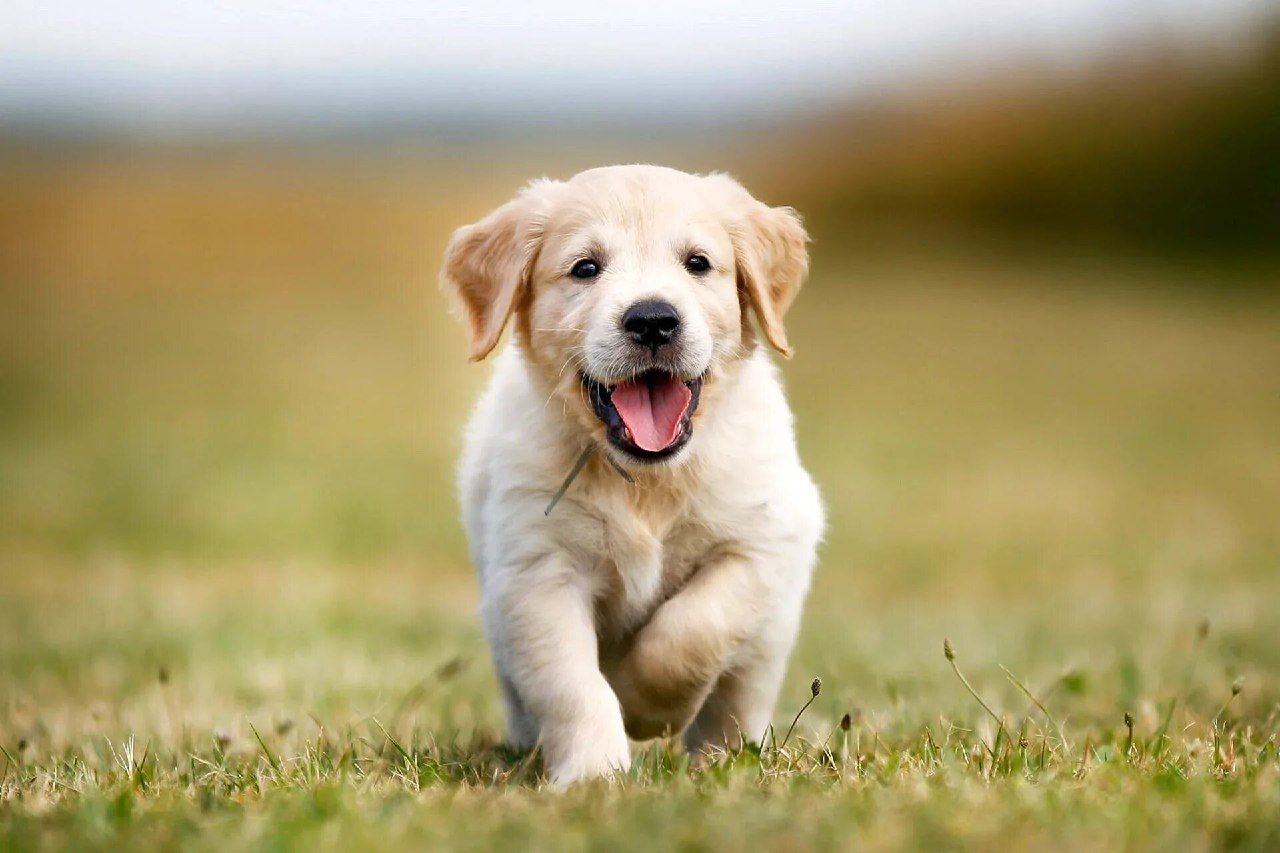
\includegraphics[width=0.5\textwidth]{imagens/dog.jpg}
    \caption{Legenda da imagem.}
    \label{fig:exemplo}
\end{figure}


\end{document}


